\documentclass[12pt]{standalone}

\usepackage{tikz}

\begin{document}
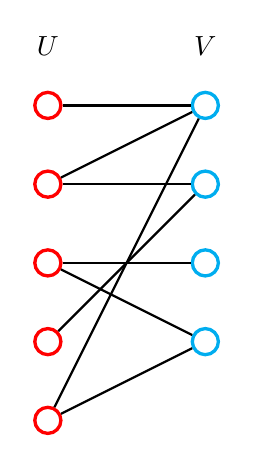
\begin{tikzpicture}

\begin{scope}[every node/.style={circle,draw,very thick,color=red}]
    \node (U0) at (0,0) {};
    \node (U1) at (0,-1) {};
    \node (U2) at (0,-2) {};
    \node (U3) at (0,-3) {};
    \node (U4) at (0,-4) {};
\end{scope}

\node at (0,0.75) {$U$};

\begin{scope}[every node/.style={circle,draw,very thick,color=cyan}]
    \node (V0) at (2,0) {};
    \node (V1) at (2,-1) {};
    \node (V2) at (2,-2) {};
    \node (V3) at (2,-3) {};
\end{scope}

\node at (2,0.75) {$V$};

\begin{scope}[thick]
    \draw (U0) -- (V0);
    \draw (U1) -- (V0);
    \draw (U1) -- (V1);
    \draw (U2) -- (V2);
    \draw (U2) -- (V3);
    \draw (U3) -- (V1);
    \draw (U4) -- (V0);
    \draw (U4) -- (V3);
\end{scope}

\end{tikzpicture}
\end{document}
